% Provenance (never printed): see sources/outline_sources.md (Year 2: viscosity, density and
% volatiles of magmas; magma ascent; dykes, sills and plutons; contact aureoles).
% Curves from figdata/bachelor-2/magma.py (GRD 2008 viscosity, DensityX density, Moore 1998
% solubility data, erf sill cooling, Stefan solidification); exercise and problem values in
% the Book 4 scratch calculators calc/ch05.py and calc/ch05pb.py.
\chapter{मैग्मा और उनका स्थापन}\label{ch:b2:magma-emplacement}

\qty{1200}{\celsius} पर एक बेसाल्टी गलित लगभग \qty{70}{Pa.s} की श्यानता के साथ बहता है:
गाढ़ा, पर वह उँडेला जा सकता है। \qty{800}{\celsius} पर एक शुष्क रायोलाइटी गलित
की श्यानता \qty{e11}{Pa.s} के निकट होती है, और उसका एक खंड अपने ही भार से दृश्य रूप से
झुकने में घंटों लेता। दोनों के बीच परिमाण की दस कोटियाँ हैं, जो
जल और बेसाल्ट के बीच के अंतर से अधिक है, और अधिकांश अंतर दो
चीज़ों से आता है: सिलिका, जो गलित को एक जाल में जोड़ती है, और तापमान,
जो सिलिसिक मैग्माओं में कई सौ डिग्री कम होता है। कुछ प्रतिशत
घुला हुआ जल, जिसे रायोलाइटी \omterm{def:b2:magma-emplacement:magma}{मैग्मा} गहराई में धारण कर सकता है, उसकी श्यानता
\num{e5} के गुणक से घटा देता है, और \omterm{def:b2:magma-emplacement:magma}{मैग्मा} के ऊपर उठने और जल के
बुलबुलों के रूप में निकलने पर यह कमी फिर खो जाती है। ये संख्याएँ तय करती हैं कि कोई \omterm{def:b2:magma-emplacement:magma}{मैग्मा}
पृष्ठ तक शांति से पहुँचता है, विस्फोट करता है, या किलोमीटरों नीचे \omterm{def:b2:magma-emplacement:bodies}{डाइक}, \omterm{def:b2:magma-emplacement:bodies}{सिल} या
\omterm{def:b2:magma-emplacement:bodies}{प्लूटॉन} के रूप में जम जाता है। यह अध्याय \omterm{def:b2:magma-emplacement:magma}{मैग्मा} को एक पदार्थ की तरह देखता है: उसका घनत्व, श्यानता और
वाष्पशील, दरारों के माध्यम से और पिंडों के रूप में उसके आरोहण की भौतिकी, रुकने पर वह जो आकार
लेता है, और आसपास की चट्टानों को वह जो ऊष्मा देता है।
% ledger: grd08:model, grd08:range, moore98:melts

\begin{recall}
\textbf{श्यान प्रवाह} (भौतिकी की पुस्तकें, द्वितीय वर्ष): श्यानता $\eta$ वाले
न्यूटनी तरल में अपरूपण प्रतिबल $\eta$ गुणा वेग-प्रवणता होता है;
दो समांतर दीवारों के बीच दाब-प्रवणता एक परवलयिक (समतल प्वाज़ॉय)
परिच्छेदिका चलाती है; श्यान तरल में धीरे चलता गोला स्टोक्स कर्षण
$6\pi\eta a v$ अनुभव करता है। \textbf{ऊष्मा चालन} (वही खंड): तापमान
$\partial T/\partial t = \kappa\,\partial^2T/\partial x^2$ का पालन करता है, जहाँ विसरणशीलता $\kappa = k/(\rho
c)$ है, और तापमान का एक सोपान त्रुटि-फलन के रूप में
$\sqrt{\kappa t}$ की कोटि की दूरी तक फैलता है। \textbf{उत्प्लावन} (भौतिकी की पुस्तकें, प्रथम वर्ष): अधिक घने तरल में
डूबा पिंड विस्थापित तरल के भार में से अपना भार घटाने के बराबर
नेट ऊर्ध्व बल अनुभव करता है। \textbf{रासायनिक साम्य} (रसायन-विज्ञान की पुस्तकें): साम्यावस्था पर
उत्पादों और अभिकारकों की सक्रियताएँ द्रव्यमान-अनुपाती क्रिया के नियम को
तापमान पर निर्भर एक स्थिरांक $K$ के साथ संतुष्ट करती हैं। इस शृंखला की पुस्तक 3 से:
शिलास्थैतिक दाब $p = \rho g z$ और भूतापीय प्रवणता; विद्यालय
खंडों से: मैफ़िक और फ़ेल्सिक चट्टानें, दीर्घक्रिस्टल और पॉर्फ़िरी गठन।
\end{recall}

\section{मैग्मा क्या है}

\begin{definition}[मैग्मा]\label{def:b2:magma-emplacement:magma}
\emph{मैग्मा}\index{मैग्मा} पृष्ठ के नीचे पिघली या आंशिक रूप से पिघली चट्टान है: एक
\emph{सिलिकेट गलित}\index{सिलिकेट गलित}, अर्थात् मुख्यतः सिलिकॉन,
ऑक्सीजन और धातु धनायनों से बना द्रव, साथ में वे क्रिस्टल और गैस-बुलबुले जो वह लिए होता है।
\emph{क्रिस्टल पंक}\index{क्रिस्टल पंक} ऐसा मैग्मा है जो क्रिस्टलों में इतना समृद्ध हो कि वे
एक-दूसरे को छूकर एक ढाँचा बनाते हैं: वह द्रव की तरह बह नहीं सकता, और उसका गलित केवल
क्रिस्टलों के बीच के रंध्रों से होकर चल सकता है।
\end{definition}

गलित का संघटन, चट्टानों की भाँति, ऑक्साइडों के भार-प्रतिशत में दिया जाता है।
पूरे अध्याय में तीन गलित संदर्भ का काम करते हैं, सभी
प्रयोगशाला में अध्ययन किए गए: मध्य-महासागरीय कटक से निकाला गया एक थोलिआइटी बेसाल्ट
(लगभग \qty{51}{\percent} SiO$_2$, \qty{12}{\percent} लौह ऑक्साइड, \qty{7}{\percent}
MgO), एक एंडेसाइट (\qty{63}{\percent} SiO$_2$) और एक रायोलाइट (\qty{78}{\percent}
SiO$_2$, \qty{8}{\percent} Na$_2$O $+$ K$_2$O और लगभग बिना लोहे या मैग्नीशियम के)।
उनके उद्गार-तापमान उनके संघटनों जितने ही भिन्न हैं: बेसाल्टी
\omterm{def:b2:magma-emplacement:magma}{मैग्मा} \qtyrange{1000}{1200}{\celsius} पर उद्गारित होते हैं (किलाउआ पर एक नली में बहते लावा का तापमान
\qty{1200}{\celsius} के निकट मापा गया है), एंडेसाइटी \omterm{def:b2:magma-emplacement:magma}{मैग्मा}
\qtyrange{800}{1000}{\celsius} पर, रायोलाइटी \omterm{def:b2:magma-emplacement:magma}{मैग्मा} \qtyrange{650}{800}{\celsius} पर।
रायोलाइटी \omterm{def:b2:magma-emplacement:magma}{मैग्मा} अधिक ठंडा होता है क्योंकि वह लंबे क्रिस्टलन का अवशेष होता है
या भूपर्पटी-चट्टानों का पहला गलित, और ये दोनों निम्न तापमान पर होते हैं
(\cref{ch:b2:magmatic-differentiation})।
% ledger: moore98:melts, tulane:magma-types, earle:kilauea-lava

क्रिस्टल-मात्रा तय करती है कि \omterm{def:b2:magma-emplacement:magma}{मैग्मा} बहता है या नहीं। बड़े ग्रेनाइट पिंडों के क्षेत्र और
भूकालानुक्रमिक अध्ययन निष्कर्ष निकालते हैं कि समग्र मैग्मीय प्रवाह के लिए आयतन से कम से कम
\qtyrange{30}{50}{\percent} गलित-अंश चाहिए; इससे नीचे
क्रिस्टल अपने पड़ोसियों से जुड़ जाते हैं और पदार्थ गलित-भरे रंध्रों वाले ठोस की तरह
विरूपित होता है। माना जाता है कि भूपर्पटी में संचित अधिकांश \omterm{def:b2:magma-emplacement:magma}{मैग्मा}
इसी अवस्था में है, एक पंक के रूप में जो नीचे से गरम \omterm{def:b2:magma-emplacement:magma}{मैग्मा} जुड़ने पर फिर
गतिशील हो जाता है।
% ledger: glazner04:tuolumne

\section{घनत्व और श्यानता}

\subsection{गलित का घनत्व}

\omterm{def:b2:magma-emplacement:magma}{सिलिकेट गलित} में कोई क्रिस्टल-जालक नहीं होता, फिर भी उसका आयतन
उसके घटकों से बनाया जा सकता है। अनेक गलितों पर प्रयोग दिखाते हैं कि हर ऑक्साइड
प्रति मोल लगभग नियत आयतन देता है, उसका आंशिक मोलर आयतन, जो
तापमान और दाब के साथ धीरे-धीरे और रैखिक रूप से बदलता है; गलित का आयतन
इन योगदानों का योग है। नीचे की तालिका इस अध्याय में प्रयुक्त मान देती है।

\begin{table}[ht]
\centering\small
\begin{tabular}{lrrr}
\hline
ऑक्साइड & $\bar V_i$ (\unit{cm^3/mol}) & $\partial\bar V_i/\partial T$ (\num{e-3}\,\unit{cm^3/(mol.K)}) & $\partial\bar V_i/\partial p$ (\num{e-4}\,\unit{cm^3/(mol.bar)}) \\
\hline
SiO$_2$  & 26.86 & 0     & $-1.89$ \\
Al$_2$O$_3$ & 37.42 & 2.62 & $-2.26$ \\
FeO      & 12.68 & 3.69  & $-0.45$ \\
MgO      & 12.02 & 3.27  & $0.27$ \\
CaO      & 16.90 & 3.74  & $0.34$ \\
Na$_2$O  & 29.65 & 7.68  & $-2.40$ \\
K$_2$O   & 47.28 & 12.08 & $-6.75$ \\
H$_2$O   & 22.9  & 9.5   & $-3.20$ \\
\hline
\end{tabular}
\caption{\omterm{def:b2:magma-emplacement:magma}{सिलिकेट गलितों} में ऑक्साइड घटकों के आंशिक मोलर आयतन,
\qty{1}{bar} पर, उनके तापमान और दाब अवकलजों के साथ। संदर्भ
तापमान \qty{1773}{K} (FeO \qty{1723}{K}, H$_2$O \qty{1273}{K})। डेटा:
DensityX प्रोग्राम का संकलन (Iacovino और Till, 2019)।}
\label{tab:b2:magma-emplacement:volumes}
\end{table}
% ledger: densityx:volumes

\begin{proposition}[सिलिकेट गलित का घनत्व]\label{prop:b2:magma-emplacement:density}
मान लीजिए किसी गलित में ऑक्साइड घटक $i$ हैं, जिनके मोल-अंश $X_i$, मोलर द्रव्यमान
$M_i$ और आंशिक मोलर आयतन $\bar V_i(T, p) = \bar V_i^{\circ} + (\partial\bar
V_i/\partial T)(T - T_{\mathrm{ref}}) + (\partial\bar V_i/\partial p)(p - p_{\mathrm{ref}})$ हैं।
यदि घटक आयतन में आदर्श रूप से मिश्रित होते हैं, तो
\[
\rho = \frac{\sum_i X_i M_i}{\sum_i X_i \bar V_i(T,p)}.
\]
\end{proposition}

\begin{proof}
गलित के एक मोल में $X_i$ मोल घटक $i$ के होते हैं, जिनका द्रव्यमान $X_iM_i$ है। आयतन में आदर्श
मिश्रण का अर्थ है कि घटक $i$ का हर मोल आयतन $\bar V_i$ जोड़ता है,
अन्य घटक जो भी हों, इसलिए गलित का मोल $\sum_i X_i\bar V_i$ घेरता है।
घनत्व इन दोनों का अनुपात है।
\end{proof}

जल का मोलर द्रव्यमान केवल \qty{18}{g/mol} है पर आंशिक मोलर आयतन
\qty{22.9}{cm^3/mol}, जो सिलिका के निकट है: वह गलित का घनत्व
प्रबल रूप से घटाता है। तीन संदर्भ गलितों पर लागू करने पर प्रतिज्ञप्ति
\qty{1200}{\celsius} पर बेसाल्ट के लिए \qty{2730}{kg/m^3}, \qty{1000}{\celsius} पर
एंडेसाइट के लिए \qty{2480}{kg/m^3} और \qty{850}{\celsius} पर शुष्क रायोलाइट के लिए \qty{2340}{kg/m^3}
देती है; एक प्रतिशत घुला हुआ जल बेसाल्ट से लगभग
\qty{70}{kg/m^3} घटा देता है, जितना कई सौ डिग्री का ऊष्मन।
इसलिए बेसाल्टी गलित उस प्रावार पेरिडोटाइट से हल्का है जिससे वह आता है
(संदर्भ पृथ्वी मॉडल में भूपर्पटी के नीचे लगभग \qty{3380}{kg/m^3}) और उस मॉडल की
निचली भूपर्पटी (\qty{2900}{kg/m^3}) से थोड़ा हल्का, जबकि
रायोलाइटी गलित उसकी ऊपरी भूपर्पटी (\qty{2600}{kg/m^3}) से भी हल्का है। यह अंतर मैग्माओं को
ऊपर की ओर धकेलता है।
% ledger: densityx:volumes, densityx:water, data:prem

\subsection{श्यानता}

\omterm{def:b2:magma-emplacement:magma}{सिलिकेट गलित} की श्यानता साझा ऑक्सीजनों से जुड़े SiO$_4$ चतुष्फलकों के जाल
से तय होती है: बहने के लिए गलित को
सिलिकॉन--ऑक्सीजन आबंध तोड़ने और फिर बनाने पड़ते हैं। सिलिका और ऐलुमिना जाल बनाते हैं;
मैग्नीशियम, लोहे, कैल्सियम और क्षारों के धनायन उसे तोड़ते हैं, और जल भी, जो
सेतु ऑक्सीजनों को हाइड्रॉक्सिल समूहों में बदल देता है। प्राकृतिक
गलितों पर प्रयोगशाला-मापन परिमाण की पंद्रह से अधिक कोटियों में फैले हैं, \qty{0.1}{Pa.s} से
\qty{e14}{Pa.s} तक, और वे सरल आरेनियस नियम का पालन नहीं करते: जैसे-जैसे गलित अपने काँच-संक्रमण
की ओर ठंडा होता है, श्यानता $1/T$ में चरघातांकी से भी तेज़
बढ़ती है।
% ledger: grd08:range

\begin{proposition}[फ़ोगेल--फ़ुल्चर--टैमान नियम]\label{prop:b2:magma-emplacement:vft}
नियत संघटन वाले \omterm{def:b2:magma-emplacement:magma}{सिलिकेट गलित} की श्यानता, लघुगणकीय इकाई के कुछ
दसवें भागों के भीतर, इसका पालन करती है:
\[
\log_{10}\eta = A + \frac{B}{T - C},
\]
जहाँ $\eta$ पास्कल सेकंड में और $T$ केल्विन में है। प्राकृतिक गलितों के लिए $A$ संघटन जो भी हो,
$-4.55$ के निकट है; $B$ और $C$ (केल्विन में) ऑक्साइडों के मोल-प्रतिशतों के रैखिक
संयोजन हैं, उनके कुछ गुणनफलों के साथ, जिन्हें लगभग \num{1800} मापनों पर
बिठाया गया है।
\end{proposition}
\admitted
% ledger: grd08:model, grd08:range

नीचे का चित्र तीन संदर्भ गलितों के लिए और घुले जल वाले
रायोलाइट के लिए यह नियम दिखाता है। \qty{1200}{\celsius} पर बेसाल्ट की
$\eta \approx \qty{70}{Pa.s}$ है; \qty{1000}{\celsius} पर एंडेसाइट की लगभग
\qty{e6}{Pa.s}; \qty{800}{\celsius} पर शुष्क रायोलाइट की लगभग $10^{10.9}$\,\unit{Pa.s}।
चार प्रतिशत जल उसी रायोलाइट को $10^{5.5}$\,\unit{Pa.s} तक नीचे ले आता है, छह
प्रतिशत $10^{4.6}$\,\unit{Pa.s} तक। केवल जलयुक्त ग्रेनाइटी गलितों पर बिठाया गया एक स्वतंत्र
समीकरण आधी लघुगणकीय इकाई के भीतर वही मान देता है
(\cref{exo:b2:magma-emplacement:1})। जल का प्रभाव निम्न तापमान पर सबसे अधिक है, जहाँ कुछ
दसवें प्रतिशत श्यानता को परिमाण की कई कोटियों से बदल देते हैं।
% ledger: grd08:model, hd96:model, moore98:melts

\begin{omfigure}
\centering
\begin{tikzpicture}
\begin{axis}[omrecord, width=0.86\linewidth, height=6.4cm,
  xmin=600, xmax=1400, ymin=0, ymax=15,
  xlabel={तापमान (\unit{\celsius})}, ylabel={$\log_{10}\eta$ (\unit{Pa.s})},
  legend pos=north east, legend style={font=\scriptsize},
  tick label style={font=\scriptsize}, label style={font=\small}]
\addplot[very thick, black, restrict x to domain=1000:1400] table[x=T_C, y=basalt] {figdata/out/bachelor-2-magma-visc.dat};
\addlegendentry{बेसाल्ट, शुष्क}
\addplot[very thick, brown, restrict x to domain=800:1300] table[x=T_C, y=andesite] {figdata/out/bachelor-2-magma-visc.dat};
\addlegendentry{एंडेसाइट, शुष्क}
\addplot[very thick, red!70!black, restrict x to domain=650:1100] table[x=T_C, y=rhyolite] {figdata/out/bachelor-2-magma-visc.dat};
\addlegendentry{रायोलाइट, शुष्क}
\addplot[thick, red!70!black, dashed, restrict x to domain=650:1000] table[x=T_C, y=rhy2] {figdata/out/bachelor-2-magma-visc.dat};
\addlegendentry{रायोलाइट, 2 \% H$_2$O}
\addplot[thick, red!70!black, densely dotted, restrict x to domain=650:1000] table[x=T_C, y=rhy4] {figdata/out/bachelor-2-magma-visc.dat};
\addlegendentry{रायोलाइट, 4 \% H$_2$O}
\addplot[thick, red!70!black, dashdotted, restrict x to domain=650:1000] table[x=T_C, y=rhy6] {figdata/out/bachelor-2-magma-visc.dat};
\addlegendentry{रायोलाइट, 6 \% H$_2$O}
\end{axis}
\end{tikzpicture}
\par\smallskip{\small तापमान के सापेक्ष \omterm{def:b2:magma-emplacement:magma}{सिलिकेट गलितों} की श्यानता,
फ़ोगेल--फ़ुल्चर--टैमान नियम से, Giordano, Russell और Dingwell (2008) के संघटन-निर्भर प्राचलों के
साथ। बेसाल्ट: एक मध्य-महासागरीय कटक थोलिआइट;
एंडेसाइट और रायोलाइट: प्रयोगशाला संदर्भ गलित (Moore और अन्य, 1998)। हर
वक्र उन तापमानों पर खींचा गया है जिन पर ऐसा \omterm{def:b2:magma-emplacement:magma}{मैग्मा} पिघला हो सकता है।}
\end{omfigure}
% ledger: grd08:model, moore98:melts

क्रिस्टल \omterm{def:b2:magma-emplacement:magma}{मैग्मा} को और भी कठोर बनाते हैं। दृढ़ कणों का निलंबन
अकेले अपने द्रव से अधिक अपरूपण का प्रतिरोध करता है, क्योंकि द्रव को कणों के चारों ओर
बहना पड़ता है, और जब कण इतने सघन हों कि एक-दूसरे को छुएँ, तो वे एक
ढाँचे में जकड़ जाते हैं।

\begin{proposition}[आइंस्टाइन--रॉस्को संबंध]\label{prop:b2:magma-emplacement:roscoe}
दृढ़ गोलों के आयतन-अंश $\phi$ का निलंबन, किसी न्यूटनी द्रव में
जिसकी श्यानता $\eta_{\ell}$ है, इस श्यानता वाला होता है:
\[
\eta = \eta_{\ell}\,(1 - R\phi)^{-2.5}, \qquad R = 1/\phi_m \approx 1.35,
\]
जहाँ $\phi_m$ अधिकतम संकुलन-अंश है, जिस पर निलंबन जाम हो जाता है।
छोटे $\phi$ के लिए यह आइंस्टाइन का $\eta = \eta_{\ell}(1 + 2.5\phi)$ बन जाता है।
\end{proposition}
\admitted
% ledger: kolz22:einstein-roscoe

बीस प्रतिशत क्रिस्टल श्यानता को दोगुना करते हैं, चालीस प्रतिशत उसे सात गुना,
साठ प्रतिशत साठ गुना से अधिक (\cref{exo:b2:magma-emplacement:5}); वास्तविक मैग्माओं में, जहाँ
क्रिस्टल लंबोतरे और अनेक आकारों के होते हैं, जकड़न पहले आती है,
क्रिस्टलों के उस \qtyrange{50}{70}{\percent} के निकट जिस पर क्षेत्रीय साक्ष्य समग्र प्रवाह का
अंत रखता है।

\section{वाष्पशील}

\begin{definition}[मैग्मीय वाष्पशील]\label{def:b2:magma-emplacement:volatiles}
\emph{मैग्मीय वाष्पशील}\index{मैग्मीय वाष्पशील} \omterm{def:b2:magma-emplacement:magma}{मैग्मा} का वह घटक है जो
गहराई में गलित में घुला रहता है और निम्न दाब पर अलग गैस प्रावस्था बनाता है:
मुख्यतः जल, फिर कार्बन डाइऑक्साइड, फिर सल्फ़र-प्रजातियाँ। \emph{वाष्पशील
निर्विलयन}\index{वाष्पशील निर्विलयन} किसी वाष्पशील का गलित से गैस के बुलबुलों में
पृथक होना है। किसी गलित का \emph{वाष्पशील संतृप्ति
दाब}\index{वाष्पशील संतृप्ति दाब} वह दाब है जिससे नीचे
उसके घुले वाष्पशील अपनी विलेयता से अधिक हो जाते हैं, जिससे गैस प्रावस्था का बनना अनिवार्य है।
\end{definition}

मैफ़िक \omterm{def:b2:magma-emplacement:magma}{मैग्मा} प्रायः द्रव्यमान से \qtyrange{1}{3}{\percent} वाष्पशील लिए होते हैं,
मध्यवर्ती \omterm{def:b2:magma-emplacement:magma}{मैग्मा} \qtyrange{3}{4}{\percent}, फ़ेल्सिक \omterm{def:b2:magma-emplacement:magma}{मैग्मा}
\qtyrange{4}{7}{\percent}, और \qtyrange{4}{6}{\percent} जल का
निर्विलयन अधिकांश विस्फोटक उद्गारों को चलाता है। कोई गलित कितना जल धारण कर सकता है, यह
सबसे बढ़कर दाब पर निर्भर करता है। नीचे का चित्र बेसाल्टी और
रायोलाइटी गलितों पर मापन दिखाता है, जिन्हें संतृप्त होने तक ज्ञात जल-दाब पर रखा गया, फिर
तेज़ी से ठंडा करके काँच बनाया गया और विश्लेषित किया गया: विलेयता निम्न दाब पर तीव्रता से और उच्च दाब पर
अधिक धीरे बढ़ती है।
% ledger: earle:volatiles, moore98:arc-water, moore98:h2o

\begin{proposition}[जल के लिए वर्गमूल नियम]\label{prop:b2:magma-emplacement:sqrt}
मान लीजिए जल \omterm{def:b2:magma-emplacement:magma}{सिलिकेट गलित} में मुख्यतः हाइड्रॉक्सिल समूहों के रूप में घुलता है,
अभिक्रिया $\mathrm{H_2O\,(gas)} + \mathrm{O^{2-}\,(melt)} \rightleftharpoons
2\,\mathrm{OH^-\,(melt)}$ द्वारा, गलित की ऑक्सीजन के बड़े आधिक्य में होने पर। तब,
निम्न जल-मात्राओं पर, घुला हुआ जल जल-दाब के वर्गमूल के
समानुपाती होता है: $w \approx s\sqrt{p}$, जहाँ $s$ गलित और
तापमान का एक स्थिरांक है।
\end{proposition}

\begin{proof}
द्रव्यमान-अनुपाती क्रिया का नियम $x_{\mathrm{OH}}^2 = K\,x_{\mathrm{O}}\,f$ देता है, जहाँ $f$
जल की फ़्यूगैसिटी है (मध्यम दाबों पर उसके दाब के निकट) और $x$
मोल-अंश हैं। गलित की ऑक्सीजन बड़े आधिक्य में है, इसलिए
$x_{\mathrm{O}}$ लगभग स्थिर रहता है, और $x_{\mathrm{OH}} = \sqrt{Kx_{\mathrm{O}}}\,
\sqrt f$। हर घुला जल-अणु दो हाइड्रॉक्सिल बनाता है, इसलिए घुला हुआ
जल $x_{\mathrm{OH}}/2$ है, $\sqrt f$ के समानुपाती। उच्चतर मात्राओं पर जल का कुछ भाग
अणुओं के रूप में घुलता है, स्वयं $f$ के अनुपात में, और
विलेयता वर्गमूल से तेज़ बढ़ती है (\cref{exo:b2:magma-emplacement:10})।
\end{proof}

मापनों पर न्यूनतम वर्गों से बिठाने पर, $w = s\sqrt p$ बेसाल्टों के लिए
$s = 0.34$ भार-प्रतिशत प्रति $\sqrt{\unit{MPa}}$ और
रायोलाइटों के लिए $s = 0.44$ देता है; हर मापन अपने वक्र से एक प्रतिशत
जल के भीतर है। तब $w$ प्रतिशत जल वाले गलित का संतृप्ति दाब
$p_s = (w/s)^2$ है: \qty{5}{\percent} जल वाले रायोलाइट के लिए \qty{129}{MPa},
भूपर्पटी में लगभग \qty{5}{km} नीचे, पर \qty{0.5}{\percent} वाले बेसाल्ट के लिए केवल
\qty{2}{MPa}, सौ मीटर या उससे कम।
% ledger: moore98:h2o

\begin{omfigure}
\centering
\begin{tikzpicture}
\begin{axis}[omrecord, width=0.8\linewidth, height=6cm,
  xmin=0, xmax=300, ymin=0, ymax=9,
  xlabel={जल-दाब (\unit{MPa})}, ylabel={घुला H$_2$O (भार \%)},
  legend pos=south east, legend style={font=\scriptsize},
  tick label style={font=\scriptsize}, label style={font=\small}]
\addplot[very thick, red!70!black] table[x=P_MPa, y=rhyolite] {figdata/out/bachelor-2-magma-solub-fit.dat};
\addlegendentry{रायोलाइट, $0.44\sqrt p$}
\addplot[only marks, mark=*, mark size=2pt, red!70!black] table[x=P_MPa, y=w] {figdata/out/bachelor-2-magma-solub-rhyolite-data.dat};
\addlegendentry{रायोलाइट, मापित}
\addplot[very thick, black] table[x=P_MPa, y=basalt] {figdata/out/bachelor-2-magma-solub-fit.dat};
\addlegendentry{बेसाल्ट, $0.34\sqrt p$}
\addplot[only marks, mark=square*, mark size=2pt, black] table[x=P_MPa, y=w] {figdata/out/bachelor-2-magma-solub-basalt-data.dat};
\addlegendentry{बेसाल्ट, मापित}
\end{axis}
\end{tikzpicture}
\par\smallskip{\small \qtyrange{800}{1200}{\celsius} पर बेसाल्टी और रायोलाइटी गलितों में
जल की विलेयता, जल-दाब के सापेक्ष: Moore और अन्य (1998) द्वारा संकलित मापन,
और न्यूनतम-वर्ग वर्गमूल नियम। \qty{100}{MPa} पर,
भूपर्पटी में लगभग \qty{4}{km} गहराई पर, रायोलाइट \qty{4.4}{\percent} जल धारण कर सकता है,
बेसाल्ट \qty{3.4}{\percent}।}
\end{omfigure}
% ledger: moore98:h2o

कार्बन डाइऑक्साइड जल से कहीं कम विलेय है। वह रायोलाइटों में अणुओं के रूप में और
बेसाल्टों में कार्बोनेट समूहों के रूप में घुलता है, थोलिआइटों की तुलना में क्षारीय गलितों में अधिक,
और उसकी विलेयता भी दाब के साथ बढ़ती है। इसलिए दोनों
गैसें लिए \omterm{def:b2:magma-emplacement:magma}{मैग्मा} गहराई में ही CO$_2$ से अत्यंत समृद्ध गैस के साथ निर्विलयन आरंभ करता है, और
\omterm{def:b2:magma-emplacement:magma}{मैग्मा} के उठने के साथ गैस जल में समृद्ध होती जाती है। गहरे समुद्र-तल पर उद्गारित
बेसाल्टों में \qty{95}{\percent} से अधिक CO$_2$ वाले आशय होते हैं, जिनके लिए
\qty{5}{km} जल के नीचे भी CO$_2$ से संतृप्ति आवश्यक थी। किलाउआ के जनक बेसाल्टों की आरंभिक
CO$_2$ मात्रा के अनुमान \qtyrange{0.2}{0.6}{\percent} तक हैं,
और उनके ओलिवीन क्रिस्टलों में फँसे गलित-अंतर्वेश \qty{500}{MPa} तक के संतृप्ति
दाब दर्ज करते हैं।
% ledger: lowenstern01:co2, lowenstern01:basalts

निर्विलयित गैस बड़ा आयतन घेरती है। \qty{900}{\celsius} पर \omterm{def:b2:magma-emplacement:magma}{मैग्मा} में एक प्रतिशत जल,
आदर्श गैस के रूप में, \qty{100}{MPa} पर आयतन का लगभग \qty{12}{\percent},
\qty{10}{MPa} पर \qty{57}{\percent} और वायुमंडलीय दाब पर
\qty{99}{\percent} से अधिक घेरता है (\cref{exo:b2:magma-emplacement:7})। बुलबुले
\omterm{def:b2:magma-emplacement:magma}{मैग्मा} का घनत्व और घटाते हैं और उसे तेज़ी से ऊपर धकेलते हैं; श्यान \omterm{def:b2:magma-emplacement:magma}{मैग्मा} में
वे निकल नहीं पाते, और \cref{ch:b2:eruptive-styles} दिखाता है कि वे उसे कैसे खंडित करते हैं।

\section{आरोहण}

अपने परिवेश से कम घना मैग्मा-पिंड प्रति एकांक आयतन
$\Delta\rho\,g$ का उत्प्लावन बल अनुभव करता है, जहाँ $\Delta\rho$ घनत्व-अंतर है। वह
दो तरह से उठ सकता है: अपने आगे खोली गई दरार से होकर, या एक गरम,
नरम पिंड के रूप में जो आसपास की चट्टान को किनारे धकेलता है।

\subsection{डाइक}

गहराई में चट्टान बड़े शिलास्थैतिक दाब के अधीन होती है, पर न्यूनतम मुख्य प्रतिबल से
थोड़े ऊँचे दाब पर \omterm{def:b2:magma-emplacement:magma}{मैग्मा} से भरी दरार अपने सिरे पर खुल
और लंबी हो सकती है। दरार के बढ़ने के साथ \omterm{def:b2:magma-emplacement:magma}{मैग्मा} उसे भरता है, और परिणाम
\omterm{def:b2:magma-emplacement:magma}{मैग्मा} की एक पतली चादर होती है, मीटरों चौड़ी और किलोमीटरों लंबी, जो अपना रास्ता काटते हुए
ऊपर बढ़ती है: बनता हुआ \omterm{def:b2:magma-emplacement:bodies}{डाइक}। तब \omterm{def:b2:magma-emplacement:magma}{मैग्मा} दो लगभग समांतर
दीवारों के बीच बहता है।

\begin{proposition}[डाइक में मैग्मा का प्रवाह]\label{prop:b2:magma-emplacement:poiseuille}
श्यानता $\eta$ वाला न्यूटनी \omterm{def:b2:magma-emplacement:magma}{मैग्मा}, जिसे दाब-प्रवणता $G$ ऊपर की ओर चलाती है
(उत्प्लावक प्रवाह के लिए, $G = \Delta\rho\,g$), दूरी $w$ पर स्थित दो समांतर दीवारों के बीच
इस माध्य वेग से बहता है:
\[
\bar u = \frac{G w^2}{12\,\eta},
\]
और \omterm{def:b2:magma-emplacement:bodies}{डाइक} की प्रति एकांक लंबाई आयतन-फ़्लक्स $q = \bar u w = G w^3/(12\eta)$ है।
\end{proposition}

\begin{proof}
स्थायी स्तरीय प्रवाह में \omterm{def:b2:magma-emplacement:bodies}{डाइक} के आर-पार वेग-परिच्छेदिका समतल
प्वाज़ॉय परवलय $u(x) = \frac{G}{2\eta}\left(\frac{w^2}{4} - x^2\right)$ है,
$-w/2 \le x \le w/2$ के लिए, जो दोनों दीवारों पर शून्य हो जाती है। इसका माध्य
$\bar u = \frac1w\int_{-w/2}^{w/2}u\,dx = \frac{G}{2\eta}\left(\frac{w^2}{4} -
\frac{w^2}{12}\right) = \frac{Gw^2}{12\eta}$ है।
\end{proof}

चौड़ाई का घन चौड़े \omterm{def:b2:magma-emplacement:bodies}{डाइकों} को संकरे \omterm{def:b2:magma-emplacement:bodies}{डाइकों} से कहीं अधिक दक्ष बनाता है।
\qty{1}{m} चौड़े \omterm{def:b2:magma-emplacement:bodies}{डाइक} में \qty{100}{Pa.s} का बेसाल्ट, $\Delta\rho =
\qty{300}{kg/m^3}$ के साथ, लगभग \qty{2.5}{m/s} से उठता है और \qty{10}{km}
भूपर्पटी एक घंटे में पार करता है; उसी \omterm{def:b2:magma-emplacement:bodies}{डाइक} में \qty{e6}{Pa.s} का रायोलाइट एक वर्ष से
अधिक लेता, और रास्ते में जम जाता, इसलिए सिलिसिक मैग्माओं को कहीं चौड़े
\omterm{def:b2:magma-emplacement:bodies}{डाइक} चाहिए (\cref{exo:b2:magma-emplacement:6})। इन प्रवाहों की रेनॉल्ड्स संख्या $\rho\bar u w/\eta$
इतनी छोटी है कि वे स्तरीय बने रहते हैं। उद्गारों के दौरान मैग्माओं की अनुमानित
आरोहण-दरें बहिःस्रावी उद्गारों, लगभग \qty{0.1}{m/s} से नीचे, को
विस्फोटक उद्गारों, उससे ऊपर, से अलग करती हैं, \qtyrange{0.005}{0.25}{m/s} की एक संक्रमणकालीन परास के साथ
जहाँ दोनों शैलियाँ होती हैं; किंबरलाइट, जो \qty{150}{km} से परे की
गहराइयों से आते हैं, \qtyrange{0.1}{30}{m/s} आँके गए हैं, और
उनमें से एक का विसरण-अध्ययन अंतिम \qtyrange{80}{110}{km} पर औसतन \qtyrange{0.02}{0.23}{m/s}
देता है, \numrange{5}{74} दिनों की यात्रा।
% ledger: cassidy18:ascent, casetta23:kimberlite

\subsection{डायापिर}

\begin{definition}[डायापिर, उदासीन उत्प्लावकता का स्तर, स्टोपिंग]\label{def:b2:magma-emplacement:ascent}
\emph{डायापिर}\index{डायापिर} उत्प्लावक पदार्थ, \omterm{def:b2:magma-emplacement:magma}{मैग्मा} या आंशिक रूप से पिघली
चट्टान, का वह पिंड है जो अपने परिवेश को किनारे बहाते हुए उसमें से ऊपर उठता है। किसी \omterm{def:b2:magma-emplacement:magma}{मैग्मा} का
\emph{उदासीन उत्प्लावकता का स्तर}\index{उदासीन उत्प्लावकता का स्तर} वह
गहराई है जिस पर उसका घनत्व आसपास की चट्टान के घनत्व के बराबर होता है: उसके नीचे
\omterm{def:b2:magma-emplacement:magma}{मैग्मा} उत्प्लावक है, उसके ऊपर अपने परिवेश से अधिक घना। \emph{मैग्मीय
स्टोपिंग}\index{मैग्मीय स्टोपिंग} दीवार या छत की चट्टान के खंडों का अलग होना है,
जो \omterm{def:b2:magma-emplacement:magma}{मैग्मा} में डूब जाते हैं; जो खंड ठोस हुई चट्टान में बंद रह जाते हैं
वे ज़ेनोलिथ हैं।
\end{definition}
% ledger: earle:intrusive-bodies

\begin{proposition}[स्टोक्स आरोहण]\label{prop:b2:magma-emplacement:stokes}
त्रिज्या $a$ और घनत्व-कमी $\Delta\rho$ वाला गोला, जो श्यानता $\eta$ वाले
न्यूटनी माध्यम में धीरे-धीरे उठ रहा हो, यह सीमांत वेग प्राप्त करता है:
\[
v = \frac{2\,\Delta\rho\,g\,a^2}{9\,\eta}
\]
यदि वह दृढ़ हो, और इसका $1.5$ गुना यदि वह नगण्य श्यानता वाला तरल हो।
\end{proposition}
\admitted

\omterm{def:b2:magma-emplacement:ascent}{डायापिर} के चारों ओर की चट्टान \qty{100}{Pa.s} का तरल नहीं बल्कि एक गरम ठोस है,
जिसकी श्यानता किसी भी गलित की श्यानता से परिमाण की कई कोटियाँ ऊँची है:
भूपर्पटी में, एक किलोमीटर चौड़ा मैग्मा-गोला प्रति वर्ष केवल मिलीमीटर उठता है, और
दूर तक उठने से बहुत पहले अपनी ऊष्मा खो देता है (\cref{exo:b2:magma-emplacement:9})। \omterm{def:b2:magma-emplacement:ascent}{डायापिर}
वहाँ काम करते हैं जहाँ परिवेश गरम और नरम हो, प्रावार में और पर्वत-पट्टियों की गहरी
जड़ों में, और जहाँ उत्प्लावक पदार्थ किलोमीटरों चौड़ा आंशिक रूप से पिघला पिंड हो;
उथली भूपर्पटी को \omterm{def:b2:magma-emplacement:bodies}{डाइक} पार करते हैं।

\section{स्थापन}

अधिकांश \omterm{def:b2:magma-emplacement:magma}{मैग्मा} कभी पृष्ठ तक नहीं पहुँचता। वह वहाँ रुक जाता है जहाँ वह उत्प्लावक नहीं रहता,
या जहाँ कोई अधिक दृढ़ परत उसे रोक देती है, और ऐसे पिंड में फैल जाता है जिसका आकार
दर्ज करता है कि उसने अपने लिए स्थान कैसे बनाया।

\begin{definition}[अंतर्वेधी पिंड]\label{def:b2:magma-emplacement:bodies}
\emph{प्लूटॉन}\index{प्लूटॉन} \omterm{def:b2:magma-emplacement:magma}{मैग्मा} का कोई भी पिंड है जो
भूपर्पटी के भीतर ठोस हुआ। \emph{डाइक}\index{डाइक} चादर जैसा प्लूटॉन है जो अपनी आतिथेय चट्टान के
स्तरण को काटता है (या कोई भी चादर, यदि आतिथेय में स्तरण न हो);
\emph{सिल}\index{सिल} स्तरण के समांतर चादर जैसा प्लूटॉन है।
\emph{लैकोलिथ}\index{लैकोलिथ} वह सिल है जो ऊपर की परतों को एक गुंबद में
उठाकर मोटा हुआ है। \emph{बैथोलिथ}\index{बैथोलिथ} एक बड़ा प्लूटॉन,
या प्लूटॉनों का समूह, है जिसका अनावृत क्षेत्रफल \qty{100}{km^2} से अधिक है।
\end{definition}
% ledger: earle:intrusive-bodies

\begin{omfigure}
\centering
\begin{tikzpicture}[x=1cm, y=1cm, font=\scriptsize]
% layered host
\fill[lith sandstone] (0,4.4) rectangle (12,5.4);
\fill[lith sandstone] (0,4.4) rectangle (12,5.4);
\fill[lith shale] (0,3.3) -- (0,4.4) -- (5.2,4.4) .. controls (5.7,4.95) and (7.0,4.95) .. (7.7,4.4)
  -- (12,4.4) -- (12,3.3) -- cycle;
\draw[thin] (0,4.4) -- (5.2,4.4) .. controls (5.7,4.95) and (7.0,4.95) .. (7.7,4.4) -- (12,4.4);
\fill[lith limestone] (0,2.2) rectangle (12,3.3);
\fill[lith sandstone] (0,0) rectangle (12,2.2);
\draw[thick] (0,0) rectangle (12,5.4);
% batholith at the bottom right
\fill[lith granite] (6.8,0) .. controls (7.2,1.6) and (8.4,2.2) .. (9.6,1.9)
  .. controls (10.6,1.7) and (11.2,1.3) .. (12,1.6) -- (12,0) -- cycle;
\draw[thick] (6.8,0) .. controls (7.2,1.6) and (8.4,2.2) .. (9.6,1.9)
  .. controls (10.6,1.7) and (11.2,1.3) .. (12,1.6);
% aureole around the batholith
\draw[densely dashed, orange!80!black, thick] (6.2,0) .. controls (6.6,2.2) and (8.4,2.8) .. (9.6,2.5)
  .. controls (10.6,2.3) and (11.3,2.0) .. (12,2.2);
% stoped blocks
\fill[lith limestone, draw=black] (8.4,1.0) rectangle (8.8,1.3);
\fill[lith sandstone, draw=black] (10.1,0.7) -- (10.5,0.8) -- (10.4,1.1) -- (10.0,1.0) -- cycle;
% feeder dyke from the bottom left, vertical
\fill[lith basalt] (2.0,0) rectangle (2.35,3.3);
\draw (2.0,0) -- (2.0,3.3) (2.35,0) -- (2.35,3.3);
% sill along shale/limestone contact
\fill[lith basalt] (2.0,3.15) rectangle (5.4,3.45);
\draw (2.0,3.15) -- (5.4,3.15) (2.35,3.45) -- (5.4,3.45);
% laccolith: lens pushing up the shale
\fill[lith basalt] (5.4,3.15) .. controls (5.6,3.95) and (6.6,4.05) .. (7.0,3.9)
  .. controls (7.3,3.8) and (7.4,3.4) .. (7.6,3.15) -- cycle;
\draw (5.4,3.45) .. controls (5.6,3.95) and (6.6,4.05) .. (7.0,3.9)
  .. controls (7.3,3.8) and (7.4,3.4) .. (7.6,3.15) -- (5.4,3.15);
% inclined dyke cutting to the surface from the laccolith
\fill[lith basalt] (6.6,3.95) -- (6.9,3.95) -- (7.6,5.4) -- (7.3,5.4) -- cycle;
% labels
\node[fill=white, fill opacity=0.8, text opacity=1, inner sep=1pt] at (1.2,1.4) {डाइक};
\draw (1.6,1.4) -- (2.0,1.4);
\node[fill=white, fill opacity=0.8, text opacity=1, inner sep=1pt] at (3.6,2.7) {सिल};
\draw (3.6,2.85) -- (3.6,3.15);
\node[fill=white, fill opacity=0.8, text opacity=1, inner sep=1pt] at (6.2,4.75) {लैकोलिथ};
\draw (6.2,4.6) -- (6.3,3.95);
\node[fill=white, fill opacity=0.8, text opacity=1, inner sep=1pt] at (9.6,0.5) {बैथोलिथ};
\node[fill=white, fill opacity=0.8, text opacity=1, inner sep=1pt, align=center] at (10.6,3.0) {संपर्क\\परिमंडल};
\draw (10.6,2.7) -- (10.8,2.3);
\node[fill=white, fill opacity=0.8, text opacity=1, inner sep=1pt, align=left] at (5.0,1.0) {स्टोपिंग से\\गिरे खंड};
\draw (5.6,1.0) -- (8.35,1.15);
\end{tikzpicture}
\par\smallskip{\small स्तरित आतिथेय में अंतर्वेधी पिंडों के आकार (व्यवस्था-चित्र, पैमाने के
अनुसार नहीं): परतों को काटता एक पोषक \omterm{def:b2:magma-emplacement:bodies}{डाइक}, संस्तर-तल के अनुदिश एक \omterm{def:b2:magma-emplacement:bodies}{सिल}, अपने ऊपर की
परतों को गुंबदाकार उठाता एक \omterm{def:b2:magma-emplacement:bodies}{लैकोलिथ}, पृष्ठ तक काटता एक \omterm{def:b2:magma-emplacement:bodies}{डाइक}, और अपनी छत से
स्टोपिंग द्वारा गिरे खंडों तथा \omterm{def:b2:magma-emplacement:aureole}{संपर्क परिमंडल} वाला एक \omterm{def:b2:magma-emplacement:bodies}{बैथोलिथ}।}
\end{omfigure}

\omterm{def:b2:magma-emplacement:magma}{मैग्मा} कहाँ रुकता है, यह सबसे पहले उसके घनत्व पर निर्भर करता है। जिस भूपर्पटी का घनत्व
गहराई के साथ बढ़ता है, उसमें \omterm{def:b2:magma-emplacement:magma}{मैग्मा} अपने उदासीन उत्प्लावकता के स्तर तक उठता है और
वहाँ किनारों की ओर फैल जाता है, \omterm{def:b2:magma-emplacement:bodies}{सिल} या लेंस के रूप में; पृष्ठ के निकट हल्के अवसाद
घने बेसाल्टी \omterm{def:b2:magma-emplacement:magma}{मैग्मा} के लिए विशेष रूप से प्रभावी जाल हैं। कोई दृढ़, कड़ी परत
भी \omterm{def:b2:magma-emplacement:bodies}{डाइक} को रोककर उसके आधार के अनुदिश मोड़ सकती है। नीचे का चित्र
सिद्धांत दिखाता है।

\begin{omfigure}
\centering
\begin{tikzpicture}[font=\scriptsize]
\begin{axis}[width=0.62\linewidth, height=6cm,
  xmin=0, xmax=1.15, ymin=0, ymax=1, y dir=reverse,
  xtick=\empty, ytick=\empty,
  xlabel={घनत्व (व्यवस्था-चित्र)}, ylabel={गहराई (व्यवस्था-चित्र)},
  label style={font=\small}, clip=false]
\addplot[very thick, black, domain=0:1, samples=40] ({0.25 + 0.55*(1 - exp(-3*x))}, {x});
\addplot[very thick, red!70!black] coordinates {(0.62,0) (0.62,1)};
\fill[red!70!black, opacity=0.15] (axis cs:0.62,0.36) rectangle (axis cs:1.15,1);
\draw[densely dashed] (axis cs:0,0.36) -- (axis cs:1.15,0.36);
\node[anchor=south west] at (axis cs:0.02,0.36) {उदासीन उत्प्लावकता का स्तर};
\node[anchor=east, black] at (axis cs:0.46,0.20) {भूपर्पटी};
\node[anchor=east, red!70!black] at (axis cs:0.61,0.85) {मैग्मा};
\node[anchor=west, align=left] at (axis cs:0.82,0.70) {मैग्मा हल्का:\\उठता है};
\node[anchor=west, align=left] at (axis cs:0.66,0.12) {मैग्मा घना:\\नीचे रुकता है};
\end{axis}
\end{tikzpicture}
\par\smallskip{\small \omterm{def:b2:magma-emplacement:ascent}{उदासीन उत्प्लावकता का स्तर} (व्यवस्था-चित्र)। भूपर्पटी का घनत्व
गहराई के साथ बढ़ता है, अवसादों के संहनन से और अधिक
घनी चट्टानों में परिवर्तन से; नियत घनत्व वाला \omterm{def:b2:magma-emplacement:magma}{मैग्मा} तब तक उठता है जब तक वह अपने
परिवेश से हल्का है (छायांकित) और जहाँ दोनों घनत्व मिलते हैं वहाँ फैल जाता है।}
\end{omfigure}

\omterm{def:b2:magma-emplacement:bodies}{प्लूटॉन} को अपने लिए स्थान बनाना पड़ता है। वह अपनी छत उठा सकता है, जैसे \omterm{def:b2:magma-emplacement:bodies}{लैकोलिथ} करता है;
जहाँ दीवारें नरम हों वहाँ उन्हें किनारे धकेल सकता है; भ्रंशन से खुले स्थान को भर सकता है;
और अपनी छत को खंड-दर-खंड स्टोप कर सकता है। बड़े \omterm{def:b2:magma-emplacement:bodies}{प्लूटॉनों} की कल्पना लंबे समय तक
एक साथ स्थापित \omterm{def:b2:magma-emplacement:magma}{मैग्मा} के विशाल टंकों के रूप में की जाती थी। आयु-निर्धारण ने वह
चित्र बदल दिया है। कैलिफ़ोर्निया के एक ग्रेनाइट \omterm{def:b2:magma-emplacement:bodies}{बैथोलिथ}, टुओलुमने अंतर्वेधी समूह, के
ज़िरकॉन दिखाते हैं कि वह \num{95} और \qty{85}{Ma} के बीच स्थापित हुआ, सबसे पुराना
किनारों पर और सबसे युवा केंद्र में, और उसकी केवल एक इकाई
\qty{3}{Myr} से अधिक में, \qty{92.8}{Ma} और \qty{88.8}{Ma} के बीच। \qty{15}{km} गहराई पर स्थापित
\qty{5}{km} मोटा और \qty{20}{km} चौड़ा \omterm{def:b2:magma-emplacement:magma}{मैग्मा} का एक अकेला पिंड
\qty{750}{\celsius} से नीचे, जहाँ वह लगभग आधा क्रिस्टलित होता है,
लगभग \num{500000}~वर्षों में ठंडा हो गया होता। ऐसे \omterm{def:b2:magma-emplacement:bodies}{प्लूटॉन} क्रमिक रूप से जोड़े गए होंगे,
चादरों और \omterm{def:b2:magma-emplacement:bodies}{डाइकों} जैसे अनेक छोटे अंतर्वेधनों से, लाखों वर्षों में
(\cref{exo:b2:magma-emplacement:11})।
% ledger: glazner04:tuolumne

\begin{omfigure}
\centering
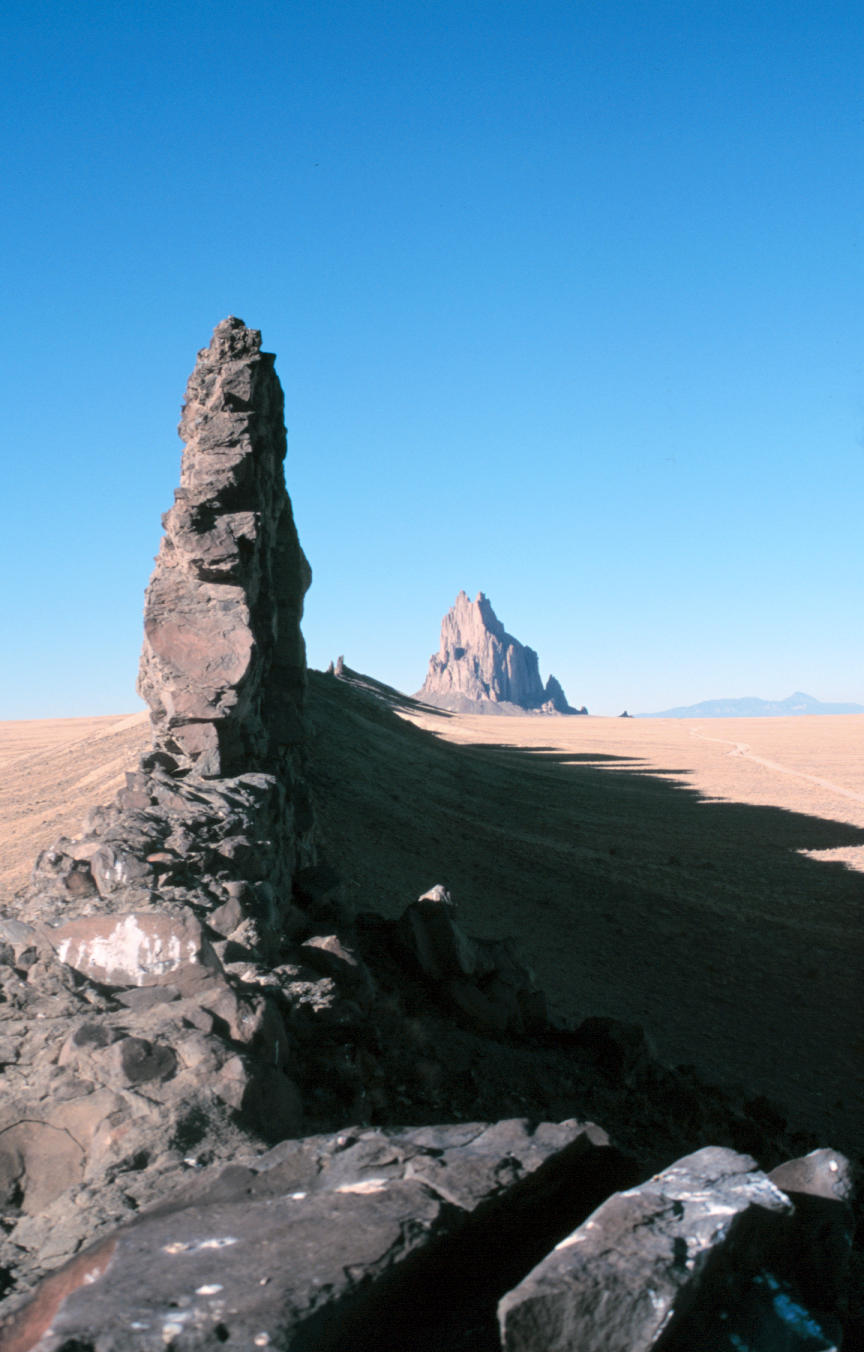
\includegraphics[width=0.3\linewidth]{images/book4/b2-shiprock-dyke.jpg}
\par\smallskip{\small नवाहो ज्वालामुखीय क्षेत्र (न्यू मेक्सिको) में शिपरॉक के निकट एक \omterm{def:b2:magma-emplacement:bodies}{डाइक}:
\omterm{def:b2:magma-emplacement:bodies}{डाइक} की चट्टान ने उस बलुआ पत्थर और शेल से बेहतर अपरदन का प्रतिरोध किया
जिसे उसने काटा था, और अब एक दीवार की तरह खड़ी है; दूर, वह ज्वालामुखीय ग्रीवा जिससे
ऐसे कई \omterm{def:b2:magma-emplacement:bodies}{डाइक} अरीय रूप से निकलते हैं। फ़ोटो: Dexter Perkins (CC0)।}
\end{omfigure}

\section{शीतलन और संपर्क कायांतरण}

अंतर्वेधन अपनी ऊष्मा चालन द्वारा अपनी आतिथेय चट्टानों में खोता है। सबसे सरल
मॉडल अंतर्वेधन और उसके आतिथेय को एकसमान विसरणशीलता $\kappa$ वाला एक चालक माध्यम मानता है:
शून्य समय पर मोटाई $b$ की एक चादर अंतर्वेधन-तापमान $T_m$ पर है और आतिथेय $T_0$ पर।
ऊष्मा-समीकरण का हल, चादर के मध्य से मापे गए
$x$ के साथ, यह है:
\[
T(x,t) = T_0 + \frac{T_m - T_0}{2}\left[\operatorname{erf}\frac{b/2 - x}{2\sqrt{\kappa t}}
+ \operatorname{erf}\frac{b/2 + x}{2\sqrt{\kappa t}}\right].
\]
नीचे का चित्र इसे \qty{100}{m} मोटी \omterm{def:b2:magma-emplacement:bodies}{सिल} के लिए दिखाता है।
% ledger: delaney86b4:properties

\begin{proposition}[संपर्क तापमान]\label{prop:b2:magma-emplacement:contact}
इस मॉडल में, जब तक $\sqrt{\kappa t}$, $b$ की तुलना में छोटा है, तब तक
अंतर्वेधन के संपर्क पर तापमान अंतर्वेधन और आतिथेय के तापमानों के माध्य $(T_m + T_0)/2$ पर
बना रहता है।
\end{proposition}

\begin{proof}
संपर्क $x = b/2$ पर पहला त्रुटि-फलन $\operatorname{erf}0 = 0$ है और
दूसरा $\operatorname{erf}(b/(2\sqrt{\kappa t}))$ है, जो $1$ के निकट रहता है जब तक
$b \gg 2\sqrt{\kappa t}$। तब $T = T_0 + (T_m - T_0)/2$।
\end{proof}

इस प्रकार \qty{50}{\celsius} की चट्टानों में \qty{1150}{\celsius} का बेसाल्टी \omterm{def:b2:magma-emplacement:bodies}{डाइक}
अपने संपर्क को \qty{600}{\celsius} तक गरम करता है। क्रिस्टलन की ऊष्मा, प्रायः
\qtyrange{700}{1000}{MJ/m^3}, \omterm{def:b2:magma-emplacement:magma}{मैग्मा} को अधिक देर तक गरम रखती है और यह मान बढ़ाती है:
\num{1150} और \qty{950}{\celsius} के बीच मुक्त \qty{900}{MJ/m^3} के साथ वही
मॉडल \qty{690}{\celsius} देता है, जबकि तापमान-निर्भर चालकताएँ और गीली
आतिथेय चट्टानें दोनों अनुमानों को 50 से \qty{75}{\celsius} घटा देती हैं।
% ledger: delaney86b4:dike, delaney86b4:properties

\begin{omfigure}
\centering
\begin{tikzpicture}
\begin{axis}[omrecord, width=0.86\linewidth, height=6cm,
  xmin=-200, xmax=200, ymin=0, ymax=1200,
  xlabel={सिल के मध्य से दूरी (\unit{m})},
  ylabel={तापमान (\unit{\celsius})},
  legend pos=north east, legend style={font=\scriptsize},
  tick label style={font=\scriptsize}, label style={font=\small}]
\fill[gray!15] (axis cs:-50,0) rectangle (axis cs:50,1200);
\addplot[very thick, red!80!black] table[x=x_m, y=t1] {figdata/out/bachelor-2-magma-sill.dat};
\addlegendentry{1 वर्ष}
\addplot[very thick, orange!90!black] table[x=x_m, y=t2] {figdata/out/bachelor-2-magma-sill.dat};
\addlegendentry{10 वर्ष}
\addplot[very thick, blue!60!black] table[x=x_m, y=t3] {figdata/out/bachelor-2-magma-sill.dat};
\addlegendentry{50 वर्ष}
\addplot[very thick, black] table[x=x_m, y=t4] {figdata/out/bachelor-2-magma-sill.dat};
\addlegendentry{200 वर्ष}
\draw[densely dashed, gray] (axis cs:-200,625) -- (axis cs:200,625);
\node[font=\scriptsize, gray!40!black, anchor=south west] at (axis cs:-198,625) {$(T_m + T_0)/2$};
\node[font=\scriptsize, anchor=south] at (axis cs:0,20) {सिल};
\end{axis}
\end{tikzpicture}
\par\smallskip{\small \qty{100}{m} मोटी \omterm{def:b2:magma-emplacement:bodies}{सिल} (छायांकित) का चालनीय शीतलन,
जो \qty{1150}{\celsius} पर \qty{100}{\celsius} की चट्टान में अंतर्वेधित हुई,
$\kappa = \qty{0.7e-6}{m^2/s}$ के साथ और बिना गुप्त ऊष्मा के। संपर्क दशकों तक
\qty{625}{\celsius} के निकट रहता है जबकि ऊष्मा आतिथेय में फैलती है; दो
शताब्दियों के बाद \omterm{def:b2:magma-emplacement:bodies}{सिल} और उसका परिवेश एक चौड़ा गरम क्षेत्र बन जाते हैं।}
\end{omfigure}
% ledger: delaney86b4:properties

शीतलन का समय-पैमाना वह समय है जो ऊष्मा को अंतर्वेधन के आर-पार विसरित होने में लगता है,
$(b/2)^2/\kappa$ की कोटि का: \qty{2}{m} चौड़े \omterm{def:b2:magma-emplacement:bodies}{डाइक} के लिए लगभग \num{16} दिन,
\qty{100}{m} मोटी \omterm{def:b2:magma-emplacement:bodies}{सिल} के लिए एक शताब्दी, कुछ किलोमीटर के \omterm{def:b2:magma-emplacement:bodies}{प्लूटॉन} के लिए एक लाख वर्ष।
गुप्त ऊष्मा इसे लंबा करती है, और \omterm{def:b2:magma-emplacement:magma}{मैग्मा} को केवल ठंडा करने के बजाय
ठोस करने की आवश्यकता भी।

\begin{proposition}[अंतर्वेधन का ठोसीकरण]\label{prop:b2:magma-emplacement:stefan}
मान लीजिए अपने ठोसीकरण-तापमान $T_m$ पर स्थित \omterm{def:b2:magma-emplacement:magma}{मैग्मा}, प्रति एकांक आयतन गुप्त ऊष्मा $L$ के साथ,
स्थान $y > 0$ को भरता है, $T_0$ पर स्थित और $y < 0$ घेरने वाली आतिथेय चट्टान के बगल में, दोनों
प्रति एकांक आयतन ऊष्मा-धारिता $\rho c$ और विसरणशीलता $\kappa$ वाले हैं।
ठोसीकरण-अग्र $y_s = 2\lambda\sqrt{\kappa t}$ के अनुसार बढ़ता है, जहाँ $\lambda$
इसका मूल है:
\[
\frac{L\sqrt\pi}{\rho c\,(T_m - T_0)} = \frac{e^{-\lambda^2}}{\lambda\,(1 + \operatorname{erf}\lambda)},
\]
और संपर्क $T_0 + (T_m - T_0)/(1 + \operatorname{erf}\lambda)$ पर रहता है। मोटाई $b$
की \omterm{def:b2:magma-emplacement:bodies}{सिल}, जो दोनों दीवारों से ठोस होती है,
$t = b^2/(16\lambda^2\kappa)$ के बाद ठोस हो जाती है।
\end{proposition}

\begin{proof}
अग्र के आगे का \omterm{def:b2:magma-emplacement:magma}{मैग्मा} $T_m$ पर रहता है, इसलिए ऊष्मा केवल ठोस
और आतिथेय में बहती है, जहाँ हम $T = T_0 + (T_m - T_0)(1 + \operatorname{erf}\xi)/(1 +
\operatorname{erf}\lambda)$ आज़माते हैं, $\xi = y/(2\sqrt{\kappa t})$ के साथ। $\xi$ का
$\alpha + \beta\operatorname{erf}\xi$ रूप वाला हर फलन ऊष्मा-समीकरण को हल करता है; यह फलन
$T_0$ की ओर प्रवृत्त होता है आतिथेय में दूर ($\xi \to -\infty$), और $T_m$ के बराबर है
अग्र $\xi = \lambda$ पर। $y = 0$ पर यह बताया गया संपर्क-तापमान देता है। अग्र पर,
आगे बढ़ते ठोस द्वारा मुक्त गुप्त ऊष्मा, $L\,dy_s/dt = L\lambda\sqrt{\kappa/t}$
प्रति एकांक क्षेत्रफल और समय, चालन द्वारा हटनी चाहिए, $k\,\partial T/\partial y = k(T_m -
T_0)\,e^{-\lambda^2}/[(1 + \operatorname{erf}\lambda)\sqrt{\pi\kappa t}]$। दोनों को बराबर रखकर
और $k = \rho c\kappa$ का प्रयोग करके $\lambda$ का समीकरण मिलता है।
\omterm{def:b2:magma-emplacement:bodies}{सिल} की हर दीवार अपना अग्र उगाती है, स्वतंत्र रूप से जब तक क्रोड $T_m$ पर रहता है; दोनों
अग्र तब मिलते हैं जब $2\lambda\sqrt{\kappa t} = b/2$।
\end{proof}

बेसाल्ट की गुप्त ऊष्मा और लगभग \qty{100}{\celsius} के आतिथेय के साथ,
$\lambda$ लगभग $0.65$ है: \qty{100}{m} मोटी \omterm{def:b2:magma-emplacement:bodies}{सिल} लगभग
सत्तर वर्षों में ठोस होती है, और इस बीच उसका संपर्क \qty{625}{\celsius} के बजाय
\qty{740}{\celsius} के निकट रहता है। सप्ताहांत समस्या इसी स्थिति पर काम करती है।
चूँकि समय मोटाई के वर्ग के साथ बढ़ता है, दस गुना मोटी \omterm{def:b2:magma-emplacement:bodies}{सिल}
सौ गुना अधिक समय लेती है।

\begin{definition}[संपर्क परिमंडल और उसकी चट्टानें]\label{def:b2:magma-emplacement:aureole}
\emph{शीतित किनारा}\index{शीतित किनारा} अंतर्वेधन का सूक्ष्म-कणिक या काचाभ किनारा है,
जहाँ \omterm{def:b2:magma-emplacement:magma}{मैग्मा} अधिक ठंडी आतिथेय चट्टान से सटकर तेज़ी से ठंडा हुआ।
\emph{संपर्क परिमंडल}\index{संपर्क परिमंडल} अंतर्वेधन के चारों ओर आतिथेय चट्टान का वह क्षेत्र है
जो उसकी ऊष्मा से कायांतरित हुआ। \emph{हॉर्नफ़ेल्स}\index{हॉर्नफ़ेल्स}
वह कठोर, सूक्ष्म-कणिक, अपर्णित चट्टान है जो पंकाश्म और ज्वालामुखीय चट्टानें
संपर्क परिमंडल में बन जाती हैं। \emph{स्कार्न}\index{स्कार्न} वह चट्टान है जो वहाँ बनती है जहाँ गरम मैग्मीय
तरल कार्बोनेट आतिथेय चट्टान से अभिक्रिया करते हैं, और गार्नेट तथा पाइरॉक्सीन जैसे कैल्सियम--लौह--मैग्नीशियम
सिलिकेट निक्षेपित करते हैं, प्रायः मैग्नेटाइट और धातु सल्फ़ाइडों के साथ।
\end{definition}
% ledger: earle:intrusive-bodies, earle:skarn

\omterm{def:b2:magma-emplacement:aureole}{संपर्क परिमंडल} छोटे \omterm{def:b2:magma-emplacement:bodies}{डाइकों} और \omterm{def:b2:magma-emplacement:bodies}{सिलों} के चारों ओर कुछ सेंटीमीटर से लेकर
किसी बड़े स्टॉक के चारों ओर कई दसियों मीटर तक होते हैं, और संपर्क कायांतरण
लगभग \qty{300}{\celsius} से \qty{800}{\celsius} से अधिक तक फैला है। पंकाश्म
\omterm{def:b2:magma-emplacement:aureole}{हॉर्नफ़ेल्स} बन जाता है, चूना-पत्थर संगमरमर, बलुआ पत्थर क्वार्ट्ज़ाइट। पहले से गरम चट्टानों में
गहराई पर स्थापित \omterm{def:b2:magma-emplacement:magma}{मैग्मा} लगभग कोई परिमंडल नहीं बनाता: चौड़ाई
अंतर्वेधन के आकार और तापमान पर और उसके आतिथेय के तापमान पर निर्भर करती है, जैसा
शीतलन मॉडल पूर्वानुमानित करता है (\cref{exo:b2:magma-emplacement:12})। परिमंडल में उगने वाले खनिज,
और वे तापमान के बारे में जो बताते हैं, \cref{ch:b2:metamorphic-facies} का विषय हैं;
\omterm{def:b2:magma-emplacement:aureole}{स्कार्न} जिन धातुओं को सांद्रित करते हैं, वे \cref{ch:b2:ore-deposits} का।
% ledger: earle:skarn

\begin{inthefield}[डाइक के संपर्कों को पढ़ना]
\begin{minipage}[t]{0.6\linewidth}\vspace{0pt}
जहाँ कोई \omterm{def:b2:magma-emplacement:bodies}{डाइक} अनावृत होता है, वहाँ भूवैज्ञानिक पहले आतिथेय चट्टान के साथ उसके संपर्कों का
अनुसरण करता है। \omterm{def:b2:magma-emplacement:bodies}{डाइक} के केंद्र से अधिक सूक्ष्म-कणिक या काचाभ किनारा दिखाता है
कि \omterm{def:b2:magma-emplacement:magma}{मैग्मा} ठंडी चट्टान से सटकर शीतित हुआ; ब्रिटिश कोलंबिया के तट पर अध्ययन किए गए
\qty{25}{cm} चौड़े एक \omterm{def:b2:magma-emplacement:bodies}{डाइक} के \omterm{def:b2:magma-emplacement:aureole}{शीतित किनारे} \qty{2}{cm} मोटे हैं। फिर
संपर्क के पास आतिथेय चट्टान की पकने के लिए जाँच की जाती है: रंग का परिवर्तन, कठोर होना,
नए खनिज जो \omterm{def:b2:magma-emplacement:bodies}{डाइक} से दूर जाते हुए धुँधले पड़ जाते हैं। पकाए गए क्षेत्र और
\omterm{def:b2:magma-emplacement:aureole}{शीतित किनारे} की चौड़ाई, \omterm{def:b2:magma-emplacement:bodies}{डाइक} की चौड़ाई के सापेक्ष मापी गई, संकेत देती है कि \omterm{def:b2:magma-emplacement:bodies}{डाइक} के
आने पर आतिथेय कितना गरम था; बिना \omterm{def:b2:magma-emplacement:aureole}{शीतित किनारे} और बिना
परिमंडल वाला \omterm{def:b2:magma-emplacement:bodies}{डाइक} पहले से गरम चट्टानों में अंतर्वेधित हुआ था। \omterm{def:b2:magma-emplacement:bodies}{डाइक} के आर-पार,
किनारे से केंद्र तक, नमूने लिए जाते हैं, उसके गलित के भू-रसायन और
उसके क्रिस्टलों के आकार के लिए।
\end{minipage}\hfill
\begin{minipage}[t]{0.36\linewidth}\vspace{0pt}
\centering
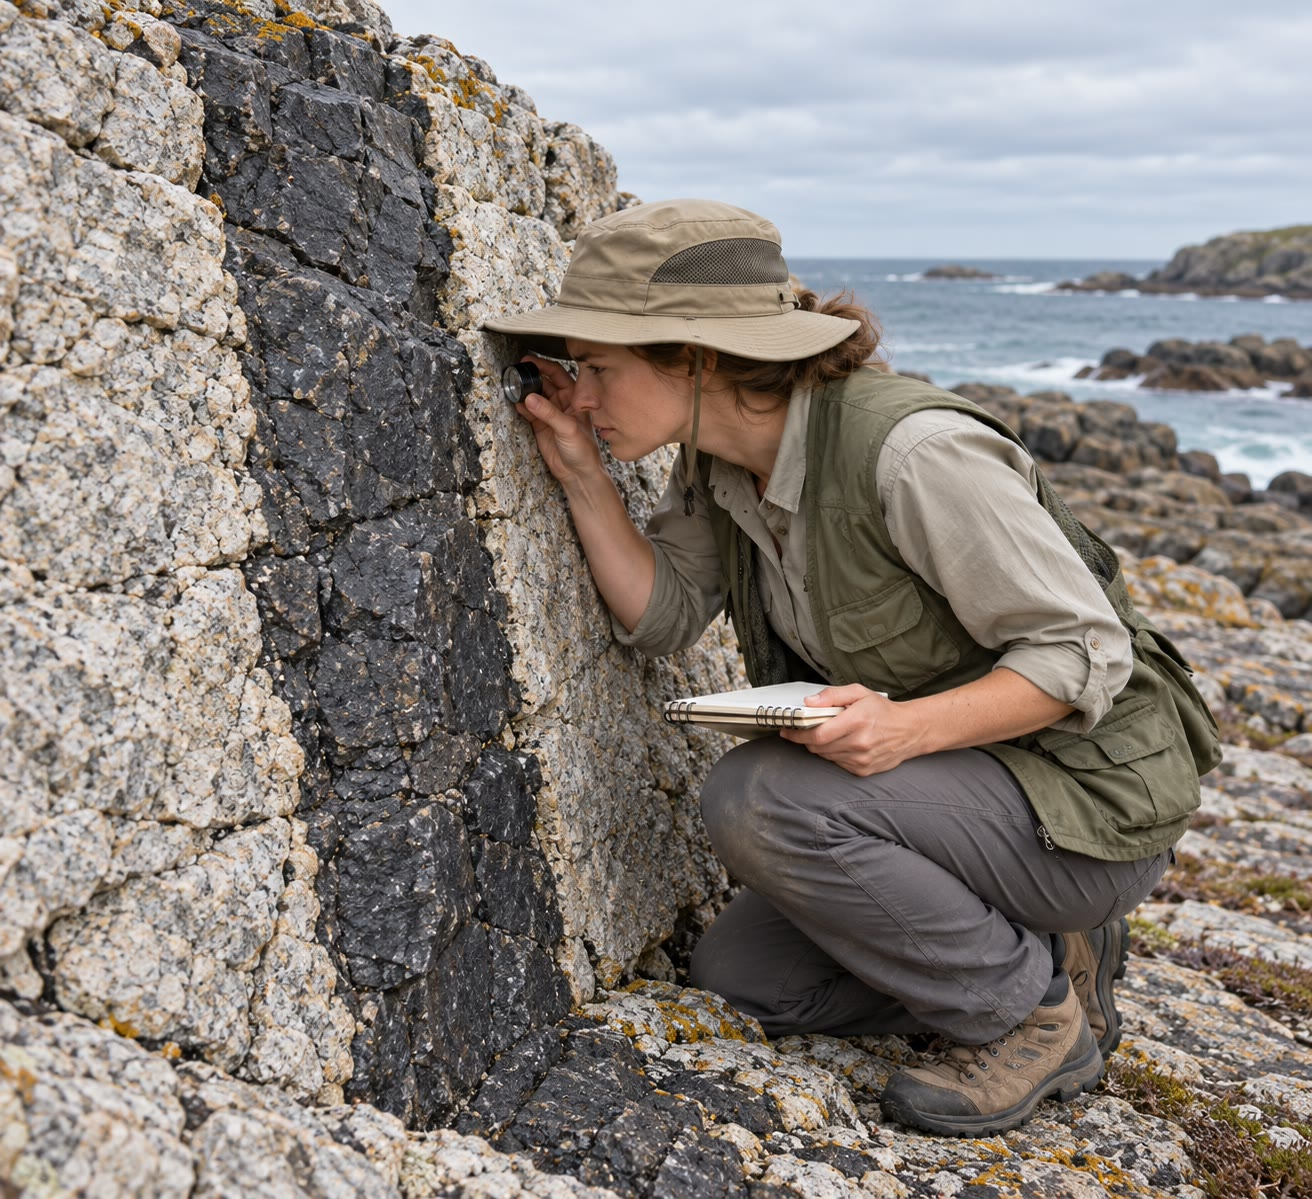
\includegraphics[width=\linewidth]{images/book4/ai/b2-dyke-contact.jpg}
\par\smallskip{\scriptsize हल्की आतिथेय चट्टान के साथ एक गहरे \omterm{def:b2:magma-emplacement:bodies}{डाइक} के संपर्क की जाँच करता
एक भूवैज्ञानिक (AI से बनाया गया चित्रण)।}
\end{minipage}
\end{inthefield}
% ledger: earle:intrusive-bodies

\section{अभ्यास}

\begin{exercise}[$\star$]\label{exo:b2:magma-emplacement:1}
जलयुक्त ग्रेनाइटी गलितों के लिए, मापनों पर बिठाया गया एक समीकरण
$\log_{10}\eta = [-3.545 + 0.833\ln w] + [9601 - 2368\ln w]/\{T - [195.7 + 32.25\ln
w]\}$ देता है, जहाँ $\eta$ \unit{Pa.s} में, $w$ भार-प्रतिशत में जल-मात्रा और $T$
केल्विन में है। \qty{800}{\celsius} पर $\log_{10}\eta$ परिकलित कीजिए, $w = 1$ और $w = 4$ दोनों के लिए,
और वह गुणक जिससे तीन अतिरिक्त प्रतिशत जल श्यानता घटाता है।
\end{exercise}
% ledger: hd96:model

\begin{exercise}[$\star$]\label{exo:b2:magma-emplacement:2}
वर्गमूल नियम से, रायोलाइट के लिए $s = 0.44$ और बेसाल्ट के लिए $s = 0.34$
(भार-प्रतिशत प्रति $\sqrt{\unit{MPa}}$) लेकर, \qty{6}{\percent} जल वाले
रायोलाइट और \qty{0.5}{\percent} वाले बेसाल्ट का संतृप्ति दाब परिकलित कीजिए,
और \qty{2600}{kg/m^3} घनत्व वाली भूपर्पटी में संगत गहराइयाँ
($g = \qty{9.81}{m/s^2}$)।
\end{exercise}

\begin{exercise}[$\star$]\label{exo:b2:magma-emplacement:3}
\qty{50}{\celsius} की चट्टानों में अंतर्वेधित \qty{1150}{\celsius} के बेसाल्टी \omterm{def:b2:magma-emplacement:bodies}{डाइक} का संपर्क-तापमान
परिकलित कीजिए, फिर \qty{400}{\celsius} की चट्टानों में।
दोनों में से किस \omterm{def:b2:magma-emplacement:bodies}{डाइक} का \omterm{def:b2:magma-emplacement:aureole}{शीतित किनारा} अधिक चौड़ा होगा?
\end{exercise}

\begin{exercise}[$\star$]\label{exo:b2:magma-emplacement:4}
हर पिंड का नाम बताइए। (क) \qty{20}{km} तक बलुआ पत्थर के दो संस्तरों के बीच पड़ी
\qty{30}{m} मोटी डोलेराइट की एक चादर। (ख) क्षैतिज चूना-पत्थरों को काटती
\qty{2}{m} चौड़ी बेसाल्ट की एक ऊर्ध्वाधर चादर। (ग) \qty{2000}{km^2} पर अनावृत एक ग्रेनाइट,
भिन्न आयुओं की दर्जन भर इकाइयों से बना। (घ) \qty{1}{km} चौड़ा पॉर्फ़िरी का एक लेंस,
आधार पर सपाट, जिसके ऊपर संस्तर मेहराब की तरह उठे हैं। (ङ) एक ग्रेनाइट में
बेसाल्ट की एक क्षैतिज चादर।
\end{exercise}

\begin{exercise}[$\star\star$]\label{exo:b2:magma-emplacement:5}
एक बेसाल्टी गलित की $\eta_{\ell} = \qty{100}{Pa.s}$ है। आइंस्टाइन--रॉस्को
संबंध ($R = 1.35$) से, \qty{5}{\percent},
\qty{20}{\percent}, \qty{40}{\percent} और \qty{60}{\percent}
क्रिस्टलों वाले \omterm{def:b2:magma-emplacement:magma}{मैग्मा} की श्यानता परिकलित कीजिए, और पहली की तुलना आइंस्टाइन के तनु सूत्र से कीजिए।
संबंध किस क्रिस्टल-अंश पर जाम पूर्वानुमानित करता है?
\end{exercise}

\begin{exercise}[$\star\star$]\label{exo:b2:magma-emplacement:6}
अपनी दीवारों से \qty{300}{kg/m^3} कम घनत्व वाला \omterm{def:b2:magma-emplacement:magma}{मैग्मा} एक \omterm{def:b2:magma-emplacement:bodies}{डाइक} से होकर उठता है।
(क) \qty{1}{m} चौड़े \omterm{def:b2:magma-emplacement:bodies}{डाइक} में बेसाल्ट ($\eta = \qty{100}{Pa.s}$, $\rho = \qty{2700}{kg/m^3}$) के लिए
माध्य वेग, \omterm{def:b2:magma-emplacement:bodies}{डाइक} के प्रति मीटर फ़्लक्स,
रेनॉल्ड्स संख्या और \qty{10}{km} उठने का समय परिकलित कीजिए। (ख) \qty{1}{m} चौड़े, फिर \qty{10}{m} चौड़े \omterm{def:b2:magma-emplacement:bodies}{डाइक} में
\qty{e6}{Pa.s} के रायोलाइट के लिए वही समय। (ग) \qty{1}{m} चौड़ा
\omterm{def:b2:magma-emplacement:bodies}{डाइक} $(w/2)^2/\kappa$ की कोटि के समय में अपनी ऊष्मा खोता है, जहाँ $\kappa =
\qty{1e-6}{m^2/s}$: तीनों में से कौन-से आरोहण सफल हो सकते हैं?
\end{exercise}

\begin{exercise}[$\star\star$]\label{exo:b2:magma-emplacement:7}
\qty{900}{\celsius} पर \qty{2400}{kg/m^3} घनत्व वाला \omterm{def:b2:magma-emplacement:magma}{मैग्मा} अपने द्रव्यमान का
\qty{1}{\percent} जलवाष्प के रूप में मुक्त करता है। वाष्प को आदर्श गैस मानकर
($R = \qty{8.314}{J/(mol.K)}$, \qty{18.015}{g/mol}), \qty{100}{MPa}, \qty{10}{MPa} और \qty{0.1}{MPa} पर \omterm{def:b2:magma-emplacement:magma}{मैग्मा} में
गैस का आयतन-अंश परिकलित कीजिए। तीनों मानों में से
कौन-सा सबसे कम विश्वसनीय है, और क्यों?
\end{exercise}

\begin{exercise}[$\star\star$]\label{exo:b2:magma-emplacement:8}
किसी द्रोणी में चट्टानों का घनत्व गहराई $z$ के साथ $\rho(z) =
2300 + 60\,z$ (\unit{kg/m^3}, $z$ \unit{km} में) के अनुसार \qty{10}{km} तक बढ़ता है। (क)
\qty{2650}{kg/m^3} के बेसाल्टी गलित का \omterm{def:b2:magma-emplacement:ascent}{उदासीन उत्प्लावकता का स्तर} कहाँ है? (ख) इस अध्याय का
घनत्व मॉडल दिखाता है कि एक प्रतिशत घुला जल बेसाल्टी गलित का घनत्व
लगभग \qty{70}{kg/m^3} घटा देता है। एक प्रतिशत अधिक जल वाला गलित कहाँ
रुकता है? (ग) अपने उदासीन उत्प्लावकता के स्तर से \qty{2}{km} नीचे शुष्क गलित पर
प्रति घन मीटर उत्प्लावन बल क्या है?
\end{exercise}

\begin{exercise}[$\star\star$]\label{exo:b2:magma-emplacement:9}
मान लीजिए त्रिज्या \qty{1}{km} और घनत्व-कमी \qty{300}{kg/m^3} वाला एक ग्रेनाइटी \omterm{def:b2:magma-emplacement:ascent}{डायापिर}
\qty{e19}{Pa.s} श्यानता वाली निचली भूपर्पटी से होकर उठता है। उसका
स्टोक्स वेग (दृढ़ गोला) मिलीमीटर प्रति वर्ष में और \qty{10}{km} उठने का समय परिकलित कीजिए।
उसके शीतलन के समय-पैमाने $a^2/\kappa$ से तुलना कीजिए, जहाँ $\kappa
= \qty{1e-6}{m^2/s}$। आप क्या निष्कर्ष निकालते हैं?
\end{exercise}

\begin{exercise}[$\star\star\star$]\label{exo:b2:magma-emplacement:10}
जल गलित में अणुओं के रूप में, $x_m = K_1 f$, और हाइड्रॉक्सिल
समूहों के रूप में, $x_{\mathrm{OH}}^2 = K_2 x_m$ (गलित की ऑक्सीजन बड़े आधिक्य में), दोनों तरह घुलता है, जिससे
कुल घुला जल $x = x_m + x_{\mathrm{OH}}/2$ है। (क) $x$ को
$f$ के फलन के रूप में व्यक्त कीजिए और दिखाइए कि वह $\sqrt f$ की तरह व्यवहार करता है निम्न $f$ पर,
और $f$ की तरह उच्च $f$ पर। (ख) किस फ़्यूगैसिटी पर जल के दोनों रूप समान रूप से प्रचुर हैं? (ग)
$K_1 = \qty{1e-4}{MPa^{-1}}$ और $K_2 = 0.2$ के साथ वह फ़्यूगैसिटी, और \qty{100}{MPa} पर हाइड्रॉक्सिल के रूप में
घुले जल का हिस्सा परिकलित कीजिए।
\end{exercise}

\begin{exercise}[$\star\star\star$]\label{exo:b2:magma-emplacement:11}
\qty{1000}{km^3} का एक ग्रेनाइट \omterm{def:b2:magma-emplacement:bodies}{प्लूटॉन} \qty{4}{Myr} में एकत्र होता है। (क)
उसकी माध्य मैग्मा-आपूर्ति \unit{km^3} प्रति वर्ष और \unit{m^3} प्रति सेकंड में परिकलित कीजिए। (ख)
\qty{1}{km} लंबा और \qty{2}{m} चौड़ा एक अकेला \omterm{def:b2:magma-emplacement:bodies}{डाइक}, \qty{0.8}{m/s} के माध्य वेग से,
उसे पोषित करता है: पूरे \omterm{def:b2:magma-emplacement:bodies}{प्लूटॉन} को पहुँचाने में \omterm{def:b2:magma-emplacement:bodies}{डाइक} कितना समय
लेगा? वह \qty{4}{Myr} का कितना अंश है? (ग) यदि \omterm{def:b2:magma-emplacement:bodies}{प्लूटॉन}
\qty{20}{m} मोटी और \qty{10}{km} गुणा \qty{10}{km} चौड़ी चादरों से बना है, तो कितनी चादरें
चाहिए, और औसतन दो चादरों के बीच कितना समय है? (घ)
$\lambda = 0.65$ और $\kappa = \qty{0.7e-6}{m^2/s}$ के साथ, एक चादर को ठोस होने में कितना
समय लगता है? क्या \omterm{def:b2:magma-emplacement:bodies}{प्लूटॉन} कभी \omterm{def:b2:magma-emplacement:magma}{मैग्मा} का एक अकेला बड़ा पिंड होता है?
\end{exercise}

\begin{exercise}[$\star\star\star$]\label{exo:b2:magma-emplacement:12}
चौड़ाई $b$ वाले एक पतले \omterm{def:b2:magma-emplacement:bodies}{डाइक} से दूर ($x \gg b$ दूरियों पर), उसकी ऊष्मा एक
तात्क्षणिक समतल स्रोत की तरह काम करती है: $T - T_0 = (T_m - T_0)\,b\,e^{-x^2/(4\kappa
t)}/\sqrt{4\pi\kappa t}$। (क) दिखाइए कि दूरी $x$ पर तापमान
$t^* = x^2/(2\kappa)$ पर सबसे ऊँचा होता है, और यह सबसे ऊँची वृद्धि $\Delta T_{\max} = (T_m -
T_0)\,b/(x\sqrt{2\pi e})$ है। (ख) $T_m - T_0 =
\qty{1100}{K}$ वाले \qty{2}{m} चौड़े \omterm{def:b2:magma-emplacement:bodies}{डाइक} के लिए, किस दूरी पर चट्टान अधिकतम \qty{100}{K} गरम होती है, और
कब ($\kappa = \qty{0.7e-6}{m^2/s}$)? (ग) पतले \omterm{def:b2:magma-emplacement:bodies}{डाइकों} के परिमंडल इतने
संकरे क्यों होते हैं?
\end{exercise}

\section{समस्या: पठार के नीचे की सिल}

\begin{problem}[{सप्ताहांत समस्या --- बेसाल्टी मैग्मा का उसके पोषक
डाइक से सिल तक अनुसरण, उसका जल, और सिल को ठोस होने में लगने वाला समय}]
\label{pb:b2:magma-emplacement:1}
एक काल्पनिक पठार के नीचे, \qty{2450}{kg/m^3} माध्य घनत्व वाले अवसाद (शेल और बलुआ पत्थर)
\qty{3.0}{km} गहराई पर \qty{2800}{kg/m^3} घनत्व वाले क्रिस्टलीय आधार पर टिके हैं।
एक बेसाल्टी \omterm{def:b2:magma-emplacement:magma}{मैग्मा} \qty{15}{km} से \qty{2.0}{m} चौड़े \omterm{def:b2:magma-emplacement:bodies}{डाइक} से होकर उठा
और अवसादों के आधार के अनुदिश \qty{100}{m} मोटी डोलेराइट \omterm{def:b2:magma-emplacement:bodies}{सिल} के रूप में फैल गया।
डेटा: अंतर्वेधन-तापमान \qty{1150}{\celsius}; गलित का
श्यानता-नियम $\log_{10}\eta = -4.55 + 5510/(T - 611)$ ($T$ केल्विन में); अपने जल सहित गलित का
घनत्व \qty{2710}{kg/m^3}; आयतन से \qty{20}{\percent} क्रिस्टल
(आइंस्टाइन--रॉस्को, $R = 1.35$); घुला जल \qty{0.40}{\percent}, विलेयता
$s = 0.34$ प्रतिशत प्रति $\sqrt{\unit{MPa}}$; \omterm{def:b2:magma-emplacement:bodies}{सिल} पर आतिथेय का तापमान
\qty{100}{\celsius}; $\kappa = \qty{0.7e-6}{m^2/s}$, $\rho c = \qty{2.5}{MJ/(m^3.K)}$,
गुप्त ऊष्मा \qty{900}{MJ/m^3}, \omterm{def:b2:magma-emplacement:magma}{मैग्मा} को उसके
अंतर्वेधन-तापमान पर ठोस होता माना जाए; $g = \qty{9.81}{m/s^2}$; एक वर्ष \qty{3.156e7}{s} है।

\medskip\noindent\textbf{भाग I --- मैग्मा।}
\begin{enumerate}
\item \qty{1150}{\celsius} (\qty{1423}{K}) पर गलित का $\log_{10}\eta$ और $\eta$
परिकलित कीजिए।
\item \qty{1100}{\celsius} पर यही। इन \qty{50}{K} में श्यानता
किस गुणक से बदलती है?
\item \qty{1150}{\celsius} पर अपने क्रिस्टलों सहित \omterm{def:b2:magma-emplacement:magma}{मैग्मा} की श्यानता
परिकलित कीजिए।
\item आइंस्टाइन--रॉस्को संबंध किस क्रिस्टल-अंश पर
\omterm{def:b2:magma-emplacement:magma}{मैग्मा} को जाम कर देगा? समग्र प्रवाह के अंत के क्षेत्रीय अनुमान से तुलना कीजिए।
\item \omterm{def:b2:magma-emplacement:magma}{मैग्मा} और आधार के बीच, और
\omterm{def:b2:magma-emplacement:magma}{मैग्मा} और अवसादों के बीच घनत्व-अंतर परिकलित कीजिए।
\item \omterm{def:b2:magma-emplacement:bodies}{सिल} के स्तर पर शिलास्थैतिक दाब परिकलित कीजिए।
\end{enumerate}

\noindent\textbf{भाग II --- डाइक में ऊपर।}
\begin{enumerate}[resume]
\item वह उत्प्लावक दाब-प्रवणता $\Delta\rho\,g$ परिकलित कीजिए जो \omterm{def:b2:magma-emplacement:magma}{मैग्मा} को
आधार में से चलाती है।
\item \omterm{def:b2:magma-emplacement:bodies}{डाइक} में \omterm{def:b2:magma-emplacement:magma}{मैग्मा} का माध्य वेग परिकलित कीजिए।
\item \omterm{def:b2:magma-emplacement:bodies}{डाइक} के प्रति मीटर फ़्लक्स, और यदि \omterm{def:b2:magma-emplacement:bodies}{डाइक} \qty{1.0}{km} लंबा है तो कुल फ़्लक्स
परिकलित कीजिए।
\item प्रवाह की रेनॉल्ड्स संख्या परिकलित कीजिए। क्या वह स्तरीय है?
\item \omterm{def:b2:magma-emplacement:magma}{मैग्मा} को \qty{15}{km} से \qty{3.0}{km} तक उठने में कितना समय लगता है?
\item उस समय-पैमाने $(w/2)^2/\kappa$ से तुलना कीजिए जिसमें \omterm{def:b2:magma-emplacement:bodies}{डाइक} अपनी
ऊष्मा खोता है। क्या वह खुला रह सकता है?
\item अध्याय की शब्दावली का प्रयोग करके समझाइए कि \omterm{def:b2:magma-emplacement:magma}{मैग्मा} \qty{3.0}{km} पर क्यों रुका और
किनारों की ओर फैला।
\end{enumerate}

\noindent\textbf{भाग III --- जल।}
\begin{enumerate}[resume]
\item गलित के जल का संतृप्ति दाब परिकलित कीजिए, और अवसादों में वह गहराई
जहाँ यह प्राप्त होता है।
\item \omterm{def:b2:magma-emplacement:bodies}{सिल} के स्तर पर गलित कितना जल धारण कर सकता था? क्या \omterm{def:b2:magma-emplacement:bodies}{सिल} का
\omterm{def:b2:magma-emplacement:magma}{मैग्मा} जल निर्विलयित करता है?
\item \omterm{def:b2:magma-emplacement:bodies}{सिल} के \omterm{def:b2:magma-emplacement:aureole}{शीतित किनारे} के आशयों में अधिकतर CO$_2$ है। समझाइए।
\item यदि सारा \qty{0.40}{\percent} जल पृष्ठ पर,
\qty{1150}{\celsius} और \qty{0.1}{MPa} पर, निकल आता, तो वाष्प \omterm{def:b2:magma-emplacement:magma}{मैग्मा} का कितना
आयतन-अंश घेरती (आदर्श गैस)?
\end{enumerate}

\noindent\textbf{भाग IV --- शीतलन और ठोसीकरण।}
\begin{enumerate}[resume]
\item गुप्त ऊष्मा की उपेक्षा करके \omterm{def:b2:magma-emplacement:bodies}{सिल} का संपर्क-तापमान परिकलित कीजिए।
\item गुप्त ऊष्मा की उपेक्षा करके, अंतर्वेधन के \num{10}~वर्ष बाद ऊपरी
संपर्क से \qty{10}{m} ऊपर तापमान परिकलित कीजिए।
\item उसी मॉडल से: \num{10}~वर्ष और \num{50}~वर्ष बाद \omterm{def:b2:magma-emplacement:bodies}{सिल} के मध्य में
तापमान परिकलित कीजिए।
\item उसी मॉडल से: ऊपरी संपर्क से \qty{80}{m} ऊपर, \num{300}, \num{363} और \num{420} वर्ष बाद
तापमान परिकलित कीजिए। क्या वहाँ की चट्टान कभी
\qty{300}{\celsius} तक पहुँचती है?
\item \omterm{def:b2:magma-emplacement:bodies}{सिल} के लिए $L\sqrt\pi/(\rho c\,(T_m - T_0))$ परिकलित कीजिए।
\item $e^{-\lambda^2}/(\lambda(1 + \operatorname{erf}\lambda))$ का मान निकालिए, $\lambda = 0.64$,
$0.65$ और $0.66$ के लिए ($\operatorname{erf}0.64 = 0.6346$, $\operatorname{erf}0.65 = 0.6420$,
$\operatorname{erf}0.66 = 0.6494$), और $\lambda$ दो दशमलव स्थानों तक बताइए।
\item गुप्त ऊष्मा सहित, \omterm{def:b2:magma-emplacement:bodies}{सिल} के ठोस होते समय संपर्क-तापमान परिकलित कीजिए। यह
प्रश्न 18 से ऊँचा क्यों है?
\item समय-पैमाना $(b/2)^2/\kappa$ वर्षों में परिकलित कीजिए।
\item \omterm{def:b2:magma-emplacement:bodies}{सिल} को ठोस होने में लगने वाला समय, वर्षों में, परिकलित कीजिए, जो इस
समस्या की मुख्य संख्या है, और समझाइए कि यह पिछले प्रश्न के समय-पैमाने से छोटा क्यों है,
यद्यपि गुप्त ऊष्मा हटानी पड़ती है।
\end{enumerate}
\end{problem}
% ledger: grd08:model, kolz22:einstein-roscoe, glazner04:tuolumne, moore98:h2o, lowenstern01:co2, delaney86b4:properties
